\section{Applied Perception}
Abbiamo visto che la visualizzazione delle informazioni consiste nel trasformare i dati in una rappresentazione 
visuale in modo che un essere umano possa estrarre informazioni utili da essi.
L'\textbf{Effectiveness} di una rappresentazione visuale non è arbitraria: ma dipende fortemente su come funziona il cervello.
Remind: l'efficacia si riferisce alla capacità di una rappresentazione visiva, come un grafico, una mappa o un diagramma, di comunicare in modo chiaro e comprensibile le informazioni desiderate. 
Capire come funziona la percezione può aiutare a prendere decisioni informate riguardo ai design delle visualizzazioni.
L'occhio umano svolge un ruolo fondamentale nella percezione visiva, essendo il principale organo sensoriale che ci consente di interpretare il mondo circostante.
L'\textbf{acuità visiva} è una misura della capacità dell'occhio di distinguere dettagli fini e di percepire chiaramente gli oggetti.
Viene spesso misurata in termini di precisione nella lettura di lettere o simboli su una tavola ottotipica posta a una certa distanza.
La nostra percezione è sensibile al contrasto di pattern, alla frequenza e all'orientamento. Inoltre, il colore influisce sulla funzione del sistema di contrasto spaziale (CSF).
Il visual Cortex è una parte del cervello che gestisce l'elaborazione delle informazioni visive provenienti dagli occhi.
\begin{figure}[H]
    \centering
    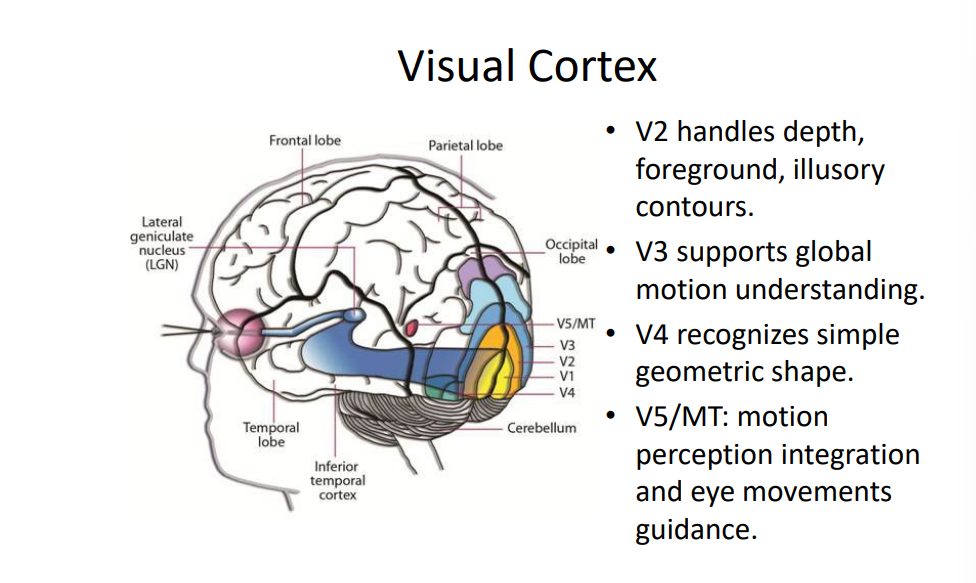
\includegraphics[width=0.5\textwidth]{images/VisualCortex.png} 
    \caption{Divisione del cervello}
    \label{fig:immagine}
\end{figure}
\subsection{Illusions}
Il campo recettivo di una cellula è l'area visiva sulla quale una cellula risponde alla luce.
Le cellule gangliari della retina sono organizzate con campi recettivi circolari.
Quando vengono stimolate al centro, vengono eccitate; quando vengono stimolate al di fuori del centro, vengono inibite.
\subsubsection{Mach Banding}
Le "Mach bands" (bande di Mach) sono un fenomeno ottico che si verifica quando si osservano transizioni tra regioni di luce e ombra su una superficie, creando 
percezioni di contrasto accentuato lungo i confini.
\subsubsection{Hermann Grid illusions}

La griglia di Hermann è un'illusione ottica che mette in evidenza l'interazione tra le cellule retiniche e il modo in cui il cervello elabora le informazioni visive. Questa illusione è composta da una griglia di linee grigie disposte a intervalli regolari, 
con dei punti neri posizionati strategicamente agli incroci delle linee.
Si ritiene che l'illusione sia causata dalla percezione del contrasto e dall'inibizione laterale nel sistema visivo. Le cellule retiniche inviano segnali al cervello che possono essere interpretati in modo errato, 
facendo percepire punti ombrosi o grigi nei punti di intersezione delle linee.
\subsubsection{Chevreul Illusion}

L'illusione di Chevreul, chiamata anche illusione dei contrasti simultanei, è un fenomeno ottico che coinvolge la percezione del colore. Questa illusione è dovuta alla sensibilità del nostro sistema visivo ai contrasti e alla relativa interpretazione dei colori circostanti.
Nell'illusione di Chevreul, se viene disegnata una serie di linee parallele in tonalità di grigio simile su uno sfondo bianco, la percezione visiva può far sembrare che i toni di grigio varino lungo le linee. Questo accade a causa dell'interazione tra i colori circostanti e la nostra percezione del contrasto.
Se due tonalità di grigio simili sono separate da una riga più chiara, il grigio sembrerà più scuro del suo vero colore. Al contrario, se sono separate da una riga più scura, sembrerà più chiaro. Questo effetto può far sembrare che i toni di grigio cambino o che vi sia un gradiente lungo le linee parallele,
 quando in realtà la differenza di colore non esiste realmente.
 \subsubsection{Greyscale Maps}
Questi effetti visivi possono portare a grandi errori quando si leggono informazioni quantitative visualizzate utilizzando una mappa in scala di grigi.
Utilizzare mappe in scala di grigi per rappresentare pochi valori (!)
\subsubsection{The Cornsweet Effect}
Le illusioni di Cornsweet sono un tipo di illusione ottica che evidenzia la percezione umana del contrasto e dei confini tra diverse superfici o tonalità. Questo tipo di illusione si basa sul modo in cui il cervello elabora i cambiamenti graduali di luminosità o colore.
Nell'illusione di Cornsweet, due aree contigue hanno un confine graduale tra loro e una transizione graduale di luminosità o colore. Nonostante la transizione sia graduale e non ci sia un cambiamento netto, la percezione visiva può far 
sembrare che ci sia un confine più netto o un cambiamento repentino.

L'effetto Cornsweet può essere utilizzato per evidenziare regioni delimitate.

Parlando dell'utilizzo delle scale di grigi, in sostanza ci sono delle regole da seguire:
Non utilizzare per mappe o per confrontare molti valori.
Utilizzare per evidenziare:
\begin{itemize}
    \item Regioni delimitate
    \item Elementi importanti (riducendo il contrasto luminoso degli elementi non importanti)
    \item Regolare la luminanza dello sfondo per ottenere una migliore leggibilità.
\end{itemize}
\subsection{Eye Movements}
\textbf{Movimenti oculari:}
\begin{itemize}
    \item \textbf{Movimenti saccadici}: movimenti balistici degli occhi che cambiano il punto di fissazione. Possono essere volontari o scatenati da stimoli.
    \item \textbf{Movimenti di inseguimento lento}: movimenti lenti degli occhi per mantenere uno stimolo in movimento sulla fovea.
    \item \textbf{Movimenti di vergenza}: allineano la fovea di ciascun occhio a un bersaglio in base alla sua distanza.
    \item \textbf{Movimenti vestibolo-oculari}: stabilizzano gli occhi compensando i movimenti della testa.

\end{itemize}
\subsection[short]{Preattentive Processes}

I processi preattentivi si riferiscono a quelle operazioni cognitive che avvengono automaticamente e
 istantaneamente nell'elaborazione delle informazioni sensoriali prima che una persona focalizzi la sua attenzione in modo consapevole su di esse. 
 Questi processi avvengono in modo rapido e automatico, senza richiedere uno sforzo cosciente.
Sono responsabili della capacità del cervello di elaborare estrarre informazioni visive, uditiva o tattili in modo veloce ed efficiente. Questi processi sono fondamentali nell'organizzazione delle informazioni sensoriali e possono avvenire a livelli inconsci della percezione umana.
Caratteristiche visive elaborate preattivamente:
\begin{itemize}
    \item Orientamento ; Curvatura ; Forma ; Dimensione ; Colore ;
    Luce/Ombra ; Contenimento ; Concavità/Convessità ;
    \item Alcune di queste non sono simmetriche.
        Caratteristiche visive non elaborate preattivamente:
        Giunzione ; Parallelismo
\end{itemize}
Alcuni processi preattentivi non sono simmetrici:
Aggiungere segni è più efficiente che rimuovere segni.
Aumentare la nitidezza è più efficiente che diminuire la nitidezza.
Un oggetto grande circondato da oggetti piccoli è più efficiente di un oggetto piccolo circondato da oggetti grandi.

\subsection{Gestalt Laws}
Le leggi della Gestalt sono principi fondamentali della psicologia della percezione che descrivono come il cervello umano organizza e interpreta le informazioni sensoriali 
per creare una percezione significativa e coerente del mondo che ci circonda. 
\begin{enumerate}
    \item \textbf{Legge della Prossimità}: Gli oggetti vicini tra loro tendono ad essere visti come parte di un insieme o di un gruppo.
    
    \item \textbf{Legge della Similarità}: Gli elementi simili per forma, colore, dimensione o altre caratteristiche tendono ad essere raggruppati insieme nella percezione.
    
    \item \textbf{Legge della Connessione}: Gli oggetti connessi sono percepiti come correlati.
        Collegare diversi oggetti con una linea è un modo efficace per esprimere che esiste una relazione tra di essi.
    
    \item \textbf{Legge della Continuità}: Gli oggetti posti lungo una linea o una curva tendono ad essere visti come parte di un modello o di un flusso continuo.
    
    \item \textbf{Legge della Simmetria}: Gli oggetti disposti simmetricamente sono percepiti come formare un insieme visivo anziché essere considerati entità separate.
     La simmetria è meglio percepita per gli assi orizzontali e verticali.
    
    \item \textbf{Legge della Chiusura}: Le persone tendono a percepire le figure incomplete come forme complete riempiendo le parti mancanti.
    
    \item \textbf{Legge della Simplicità o della Buona Forma}: La percezione tende a organizzare gli stimoli in modo da formare figure semplici e coerenti piuttosto che configurazioni disordinate o complesse.
    
    \item \textbf{Legge della Destinzione Figure-Ground}: Gli oggetti possono essere percepiti come figure distinte rispetto al loro sfondo circostante.
    
    \item \textbf{Legge del Movimento Comune}: Gli oggetti che si muovono nella stessa direzione o seguendo lo stesso modello di movimento possono essere percepiti come parte di un unico oggetto o gruppo.
  \end{enumerate}
  \subsection{Illusions}
  \subsubsection{Muller-Lyer}
  Queste due linee hanno lunghezze uguali ma vengono percepite di lunghezze diverse.
    \begin{itemize}
        \item Due spiegazioni:
        \begin{enumerate}
            \item Spiegazione prospettica
            \item Spiegazione del baricentro
        \end{enumerate}
    \end{itemize}
  \subsubsection{Wundt}
  Queste illusioni coinvolgono principalmente la percezione delle dimensioni, delle proporzioni e delle distanze tra gli oggetti, portando
   a percezioni distorte o erronee della realtà visiva.
  \subsubsection{Hering}
  Un'altra illusione simile (effetto invertito dell'illusione di Wundt).
\begin{itemize}
    \item Possibili spiegazioni:
    \begin{enumerate}
        \item Inibizione laterale
        \item Effetto prospettico
        \item Ritardi temporali nell'elaborazione visiva
    \end{enumerate}
\end{itemize}

  \subsubsection{Horizontal–Vertical Illusion}
  Un'altra semplice illusione scoperta da Wundt.
  La linea verticale viene percepita come lunga al 30\% in più rispetto alla linea orizzontale.
  Sono state osservate differenze (piccole) tra le culture.
  Questo vale anche per le linee che si intersecano.
  \subsubsection{Comparing Area}
  Confrontare le aree è difficile (ricordare le aree dei cerchi appena menzionate).
    \begin{itemize}
        \item Quando confrontiamo le aree, le proporzioni sono sottovalutate (peggio per i volumi).
        \item Flannery (1970) propose di compensare la percezione applicando un fattore di scala percettiva.
        \item Tufte, nel suo famoso libro "The Visual Display of Quantitative Information" (2001), si oppose a qualsiasi cosa tranne che l'uso di una scala assoluta, ovvero esclude la compensazione per le mancanze percettive umane.
    \end{itemize}
    La scalatura percettiva potrebbe essere insufficiente. Le cose sono più complesse da un punto di vista percettivo
